\documentclass{article}
\usepackage{graphicx} % Required for inserting images
\usepackage{float}
\usepackage[T1]{fontenc}
\usepackage{amsmath}
\usepackage[margin=1in]{geometry}
\usepackage{booktabs}
\usepackage{tabularx}
\usepackage[hidelinks]{hyperref}

\title{Always short a 25-delta put, ignoring the VRP signal}
\author{Experiment report \textperiodcentered{} L/S Gamma Desk, QUANTT}
\date{2026-10-17}

\begin{document}

\maketitle

\textbf{Question:} On the 25-delta short-put book with the 10-share hedge band, does being short every day regardless of the VRP signal raise net P\&L over the signal-timed book, at 1x and 2x spreads, in both halves, without a worse daily tail?

\textbf{Method:}

\begin{itemize}

\item \textbf{Pre-registration:} the hypothesis card was committed before any run (commit 4e3e599). No engine code was added.

\item \textbf{Data:} the paper rules (\texttt{configs/\allowbreak{}paper.\allowbreak{}toml}), with the changes below, are replayed on R2 replay snapshots v1 (config\_hash b040760187f0) over the development window 2014-06-02 to 2024-12-31. The hold-out (2025-01-01 to 2026-07-10) was not used.

\item \textbf{Book:} short-only, a 25-delta short put (\texttt{[backtest] put\_\allowbreak{}delta = 0.\allowbreak{}25}), the 10-share hedge band, and hedges once a day at 10:15 ET.

\item \textbf{The change:} \texttt{[signal] short\_\allowbreak{}band = -\allowbreak{}inf}. The signal is always short, the flat exit cannot fire, and the book re-enters on the same run after every exit, so it rolls continuously. The 7-DTE time exit, the 1x-credit stop, the 50\% profit-take and the 1-day cool-off are the live values, unchanged; the backtest's pre-hold-out embargo also applies.

\item \textbf{Variants:} \texttt{always25} (primary), and \texttt{always\_\allowbreak{}atm} (sensitivity, reported only: the same rules with the ATM put).

\item \textbf{Reference:} the registered \texttt{2026-\allowbreak{}10-\allowbreak{}17-\allowbreak{}otm-\allowbreak{}put/\allowbreak{}put25} runs (signal-timed 25-delta put), reused, not rerun. Baseline trial 1 is shown for context.

\item \textbf{Runs:} every variant ran once at 1x and 2x spreads. Costs are \$0.65 per contract and \$0.005 per share, with a \$1 minimum per order.

\end{itemize}

This report was written by Claude at the PM's request.

\section{Result vs the pass bar}

\texttt{always25} against \texttt{put25} at the same spread multiple. P\&L is net USD on daily equity for 1 contract. ES is the mean of the worst 5\% of daily P\&L, over all days.

\begin{center}\small
\begin{tabularx}{\linewidth}{>{\raggedright\arraybackslash}X l l l l l}
\toprule
\textbf{Check} & \textbf{1x value} & \textbf{1x bar} & \textbf{2x value} & \textbf{2x bar} & \textbf{Result} \\
\midrule
Net P\&L, full window & +1,316 & > +180 & +862 & > \ensuremath{-}273 & pass \\
Net P\&L, 2014-06 to 2019-12 & +553 & > \ensuremath{-}280 & +371 & > \ensuremath{-}410 & pass \\
Net P\&L, 2020-01 to 2024-12 & +763 & > +460 & +491 & > +137 & pass \\
abs ES 5\% \ensuremath{\leq} 1.10 \ensuremath{\times} reference & 121.2 & \ensuremath{\leq} 79.2 & 123.8 & \ensuremath{\leq} 80.5 & \textbf{fail} \\
Event floor: round trips (1x) & 187 & \ensuremath{\geq} 30 &  &  & met \\
\bottomrule
\end{tabularx}
\end{center}

\textbf{Verdict: failed}, on the tail guard only: the daily ES is 1.68x the reference's at 1x and 1.69x at 2x. Every P\&L check passes, in both halves and at both spreads. \texttt{always25} is the first book in the desk's backtests with positive net P\&L at 2x spreads (+\$862). The PM chose before the run to keep the ES limit at 1.10x.

\subsection{Full-window numbers (not part of the bar)}

\begin{center}\small
\begin{tabularx}{\linewidth}{>{\raggedright\arraybackslash}X l l >{\raggedright\arraybackslash}X l l >{\raggedright\arraybackslash}X}
\toprule
\textbf{} & \textbf{put25 1x} & \textbf{always25 1x} & \textbf{always\_atm 1x} & \textbf{put25 2x} & \textbf{always25 2x} & \textbf{always\_atm 2x} \\
\midrule
Net P\&L & +180 & \textbf{+1,316} & \ensuremath{-}845 & \ensuremath{-}273 & \textbf{+862} & \ensuremath{-}3,812 \\
Sharpe on \$250k & +0.04 & +0.19 & \ensuremath{-}0.10 & \ensuremath{-}0.06 & +0.12 & \ensuremath{-}0.45 \\
Max drawdown & 1,237 & 2,041 & 3,589 & 1,431 & 2,195 & 5,280 \\
ES 5\% (daily, all days) & \ensuremath{-}72.0 & \ensuremath{-}121.2 & \ensuremath{-}142.1 & \ensuremath{-}73.2 & \ensuremath{-}123.8 & \ensuremath{-}157.7 \\
Days holding a position & 27\% & 99\% & 99\% &  &  &  \\
Round trips & 105 & 187 & 178 & 105 & 187 & 178 \\
Hedge orders & 340 & 609 & 850 & 340 & 607 & 848 \\
\bottomrule
\end{tabularx}
\end{center}

\subsection{P\&L by window (not part of the bar)}

\begin{center}\small
\begin{tabularx}{\linewidth}{>{\raggedright\arraybackslash}X l l >{\raggedright\arraybackslash}X l l >{\raggedright\arraybackslash}X}
\toprule
\textbf{Window} & \textbf{put25 1x} & \textbf{always25 1x} & \textbf{always\_atm 1x} & \textbf{put25 2x} & \textbf{always25 2x} & \textbf{always\_atm 2x} \\
\midrule
2014-06 to 2015-05 & +85 & +413 & +256 & +77 & +386 & +102 \\
2015-06 to 2021-12 (archive window) & +761 & +1,361 & +1,707 & +428 & +1,022 & +227 \\
2022 & \ensuremath{-}1,039 & +16 & \ensuremath{-}1,576 & \ensuremath{-}1,123 & \ensuremath{-}211 & \ensuremath{-}2,387 \\
2023-2024 & +374 & \ensuremath{-}475 & \ensuremath{-}1,231 & +345 & \ensuremath{-}335 & \ensuremath{-}1,754 \\
\bottomrule
\end{tabularx}
\end{center}

\section{Charts}

\begin{figure}[H]\centering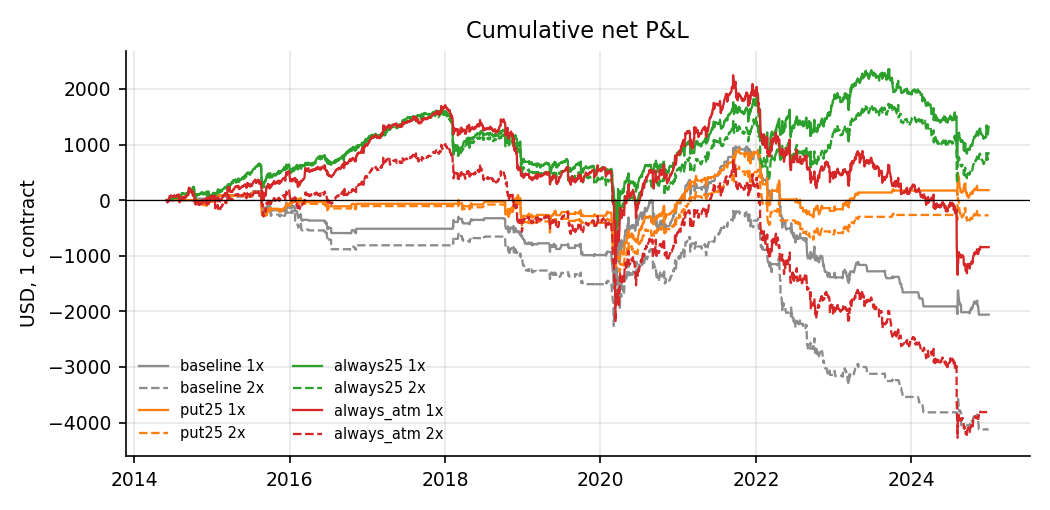
\includegraphics[width=0.92\linewidth]{figures/cum_pnl.png}\caption{Cumulative net P\&L, 1x solid and 2x dashed; baseline (live rules) grey}\end{figure}

\texttt{always25} (green) rises steadily from 2014 to early 2018, where the timed books are flat or falling. It ends 2017 at +\$1,597 at 1x, against \ensuremath{-}\$66 for the timed book. It gives part of that back in 2018 and the March 2020 crash, then peaks at +\$2,355 in September 2023. The ATM version (red) tracks it until 2021, then falls hard in 2022 and 2024.

\begin{figure}[H]\centering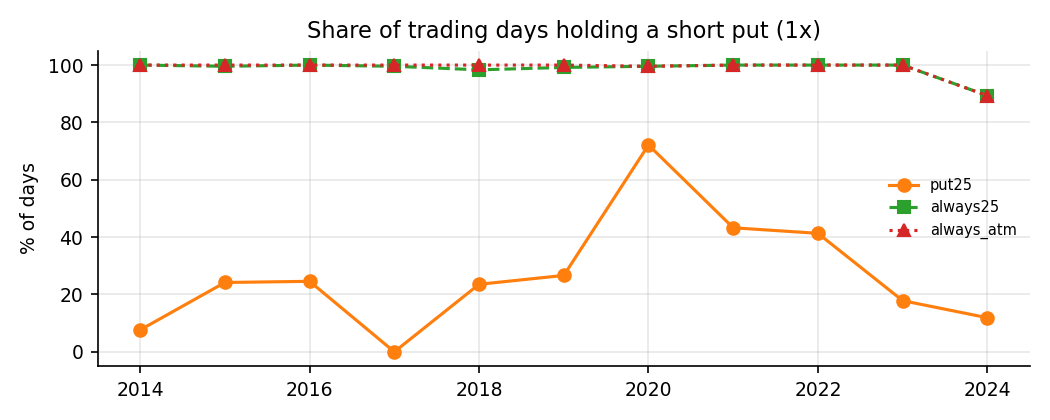
\includegraphics[width=0.92\linewidth]{figures/exposure.png}\caption{Share of trading days holding a short put}\end{figure}

This chart is the experiment. The timed book holds a position on 27\% of days, from 0\% in 2017 to 72\% in 2020. The always-short books hold one on 99\% of days. The dip to 89\% in 2024 is the embargo: no entries in the last 45 days before the hold-out.

\begin{figure}[H]\centering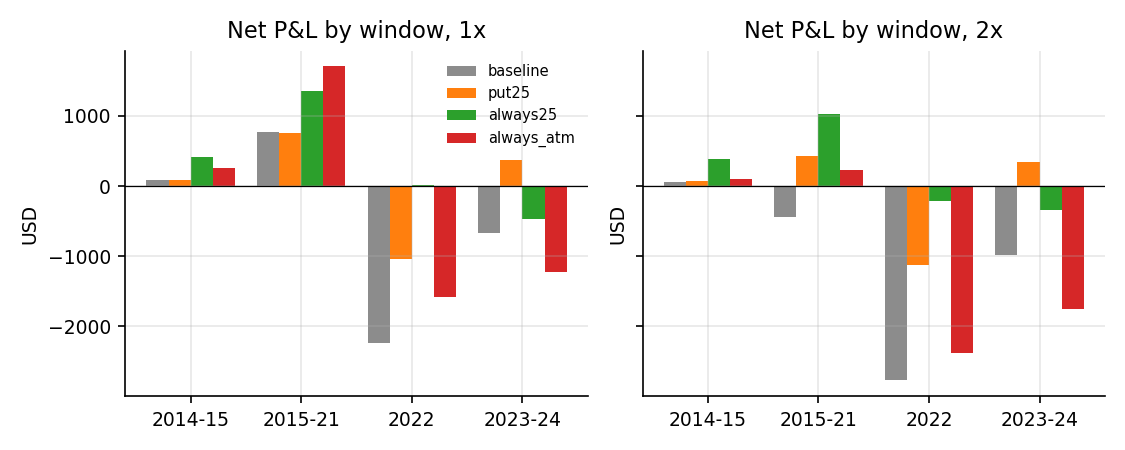
\includegraphics[width=0.92\linewidth]{figures/windows.png}\caption{Net P\&L by window}\end{figure}

Always-short wins in every window except 2023-2024. In 2015-2021, the archive's window, it makes +\$1,361 at 1x. In 2022 it roughly breaks even (+\$16 at 1x), where the timed book lost \$1,039: the timed book was short in the worst stretches of the sell-off, while the rolling book also collected premium on the days in between. 2023-2024 loses \$475 at 1x, mostly in the August 2024 spike.

\begin{figure}[H]\centering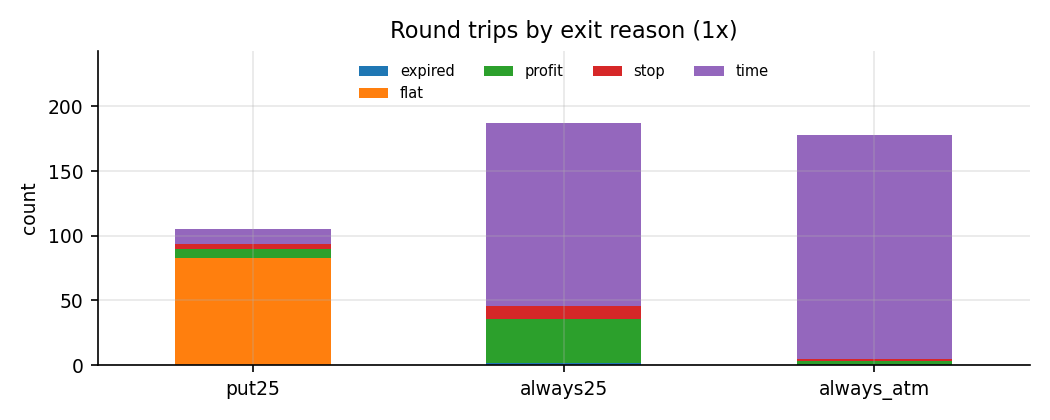
\includegraphics[width=0.92\linewidth]{figures/exits.png}\caption{Round trips by exit reason}\end{figure}

The rolling book closes 141 trades at the time exit, takes profit 34 times (+\$3,710), is stopped 10 times (\ensuremath{-}\$3,119) and holds 2 to expiry. The timed book closed most of its trades on the flat signal.

\begin{figure}[H]\centering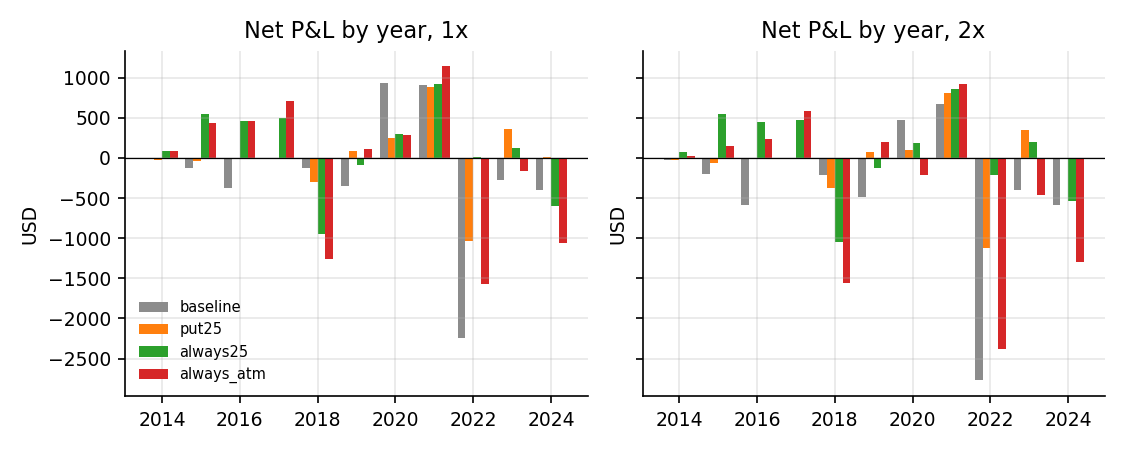
\includegraphics[width=0.92\linewidth]{figures/yearly.png}\caption{Net P\&L by year}\end{figure}

At 1x \texttt{always25} makes money in 2014-2017 (+\$1,597 together, against \ensuremath{-}\$66 for the timed book), 2020, 2021, 2022 and 2023. It loses in 2018 (\ensuremath{-}\$953, in February and December), 2019 (\ensuremath{-}\$91) and 2024 (\ensuremath{-}\$597).

\begin{figure}[H]\centering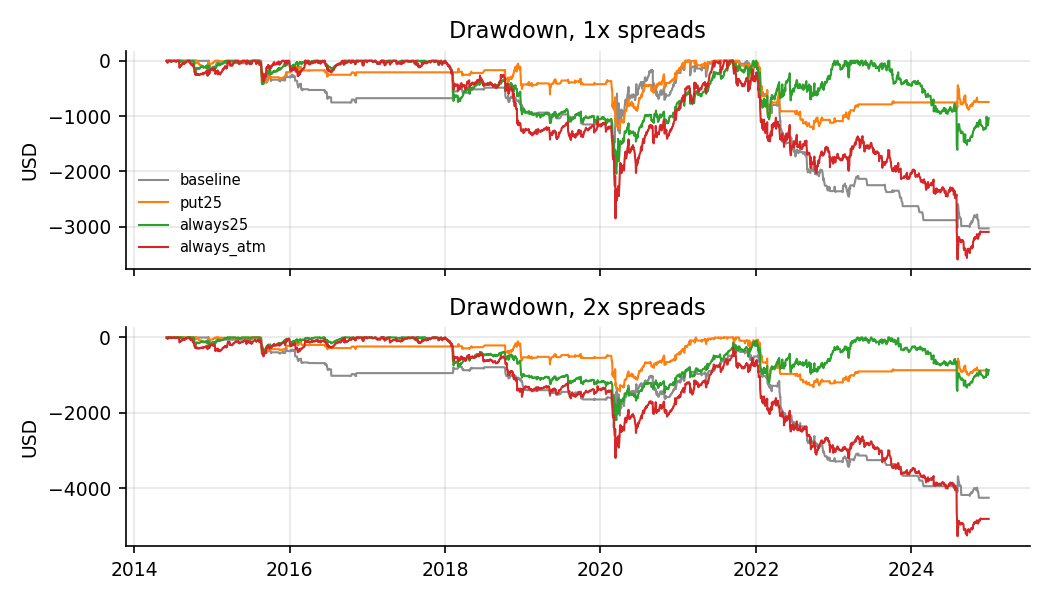
\includegraphics[width=0.92\linewidth]{figures/drawdown.png}\caption{Drawdown at 1x and 2x spreads}\end{figure}

The maximum drawdown is larger: \$2,041 against \$1,237 at 1x, with the trough at the March 2020 crash (2020-03-16). It is still smaller than the live baseline's \$3,027.

\begin{figure}[H]\centering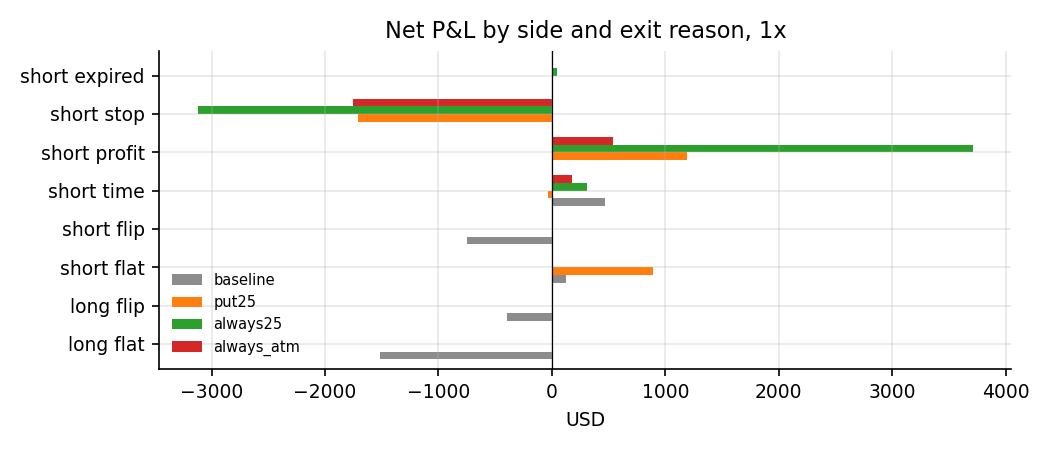
\includegraphics[width=0.92\linewidth]{figures/by_reason.png}\caption{Net P\&L by side and exit reason, 1x}\end{figure}

Profit-takes and stops net +\$591, more than the time exits (+\$310 net). Round trips add up to \$946 of the \$1,316 equity P\&L at 1x. The other \$370 sits outside any round trip, most likely shares left inside the 10-share band and the hedge unwinds.

\begin{figure}[H]\centering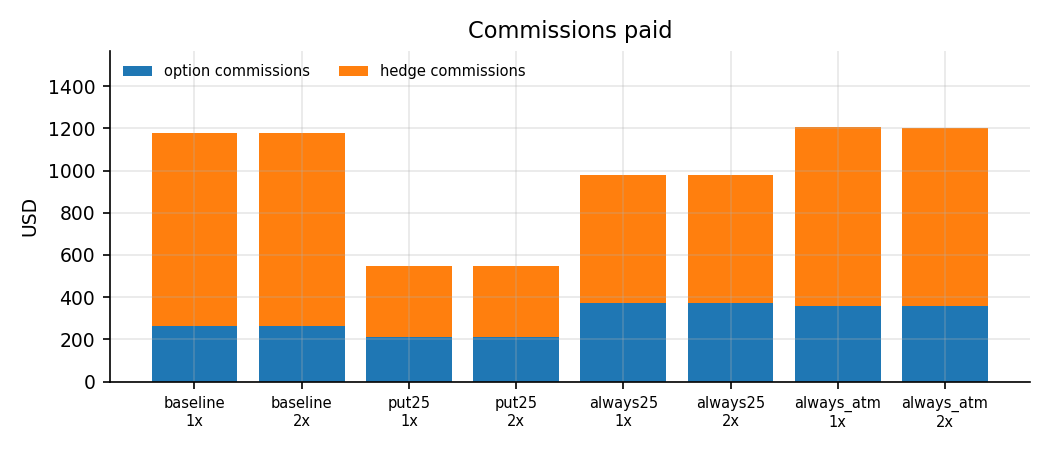
\includegraphics[width=0.92\linewidth]{figures/fees.png}\caption{Commissions paid}\end{figure}

Commissions rise from \$550 to \$981, because the book trades about 1.8 times as many round trips and hedges almost every week.

\section{Analysis}

\begin{itemize}

\item \textbf{Sitting out cost more than it saved.} Being short every day beats being short only when the signal says so, on every P\&L check, at both spreads. Before costs the rolling book earns about +\$2,750 against +\$1,183. The gap comes from the years the signal mostly sat out: in 2014-2017 the rolling book made +\$1,597 against \ensuremath{-}\$66, which is more than the whole net gap (+\$1,136). From 2018 to 2024 the rolling book is \$527 behind. The archived v1 backtest pointed the same way, but it inspired this test, so the agreement is weak evidence.

\item \textbf{The bigger tail is real, not just more exposure.} Daily ES over all days is \ensuremath{-}\$121 against \ensuremath{-}\$72, and part of that is the timed book being flat 73\% of the time. But compare the two books on the same 800 days the timed book was exposed. There the rolling book's ES is \ensuremath{-}\$167 against \ensuremath{-}\$136, and it lost \$1,089 where the timed book made \$180. All of the rolling book's profit (+\$2,405) came on the days the timed book was flat, where its ES is \ensuremath{-}\$92. So the signal's short days were bad days to be short, and the rolling book is riskier than the timed book on exactly those days.

\item \textbf{The 25-delta strike still matters.} The ATM version (\texttt{always\_\allowbreak{}atm}) earns more before costs (+\$3,328) but pays \$2,967 in spreads against \$453, and loses at both spreads. This repeats the \texttt{2026-\allowbreak{}10-\allowbreak{}17-\allowbreak{}otm-\allowbreak{}put} finding: ATM closes, especially deep in the money, are expensive in the spread model.

\item \textbf{2022 is the surprise.} The timed book lost \$1,039 in 2022; the rolling book broke even. In 2022 the rolling book lost \$942 on the days the timed book was short and made \$958 on the rest, so spreading the exposure across the year is what saved it. Why the signal picked bad days (for example the GARCH forecast lagging in the sell-off) is not tested here.

\item \textbf{The tail is spread over the stress years.} The rolling book's worst 5\% of days fall mostly in 2022 (30 days), 2020 (22), then 2024, 2018 and 2023. 60 of its 129 tail days are also in the timed book's tail. The worst day is \ensuremath{-}\$677 on 2024-08-02 (a stop). The losing years are 2018 (February and December), 2019 and 2024.

\end{itemize}

\section{Verdict}

\textbf{Failed} on the pre-registered bar, on the tail guard only (ES 1.68x the reference at 1x and 1.69x at 2x). The P\&L hypothesis held clearly. Not promoted. The ES limit was set before the run and kept by the PM, so it is not changed now.

What this means for the desk: the most profitable book so far, and the only one positive at 2x, is the simplest. It is always short a 25-delta put, hedged with a 10-share band. Whether its tail is acceptable is a risk decision for the PM, and it is not answered by re-testing this card. Possible follow-ups, each needing its own card (all in-sample, each adding trials):

\begin{itemize}

\item \textbf{A risk-adjusted bar:} compare the two books on a pre-registered risk-adjusted measure, e.g. P\&L per unit of ES. ES on held days does not rescue the rolling book: on the timed book's exposed days it is the riskier of the two.

\item \textbf{Skip the signal's short days:} the signal's short days were the worst days to be short. A rolling book that stays out on those days, using the band as an upper limit instead of a trigger, is a direct test, and it needs a small backtest switch. A stress filter in the VIX-gate style is less promising here: 60 of the rolling book's 129 tail days are also in the timed book's tail, where the VIX gate already failed (\texttt{2026-\allowbreak{}10-\allowbreak{}16-\allowbreak{}vix-\allowbreak{}gate-\allowbreak{}backtest}).

\item \textbf{Further out of the money (15-20 delta) on the rolling book.}

\end{itemize}

\section{Caveats}

\begin{itemize}

\item \textbf{In-sample:} the idea comes from the desk's review of the baseline signal and from the archived v1 results, which cover 2015-2021 (inside this window). The proxy test in \texttt{2026-\allowbreak{}10-\allowbreak{}07-\allowbreak{}garch-\allowbreak{}bias-\allowbreak{}correction} warned that shorting more often adds tail losses, and the tail result here agrees.

\item \textbf{Spread model:} fitted on about two weeks of calm 2026 live quotes. The OTM-vs-ATM cost gap drives part of the result, and real paper-account fills should be checked against it.

\item \textbf{Exposure:} the rolling book is short on almost every day, so it depends on the volatility risk premium staying positive. Over 2014-2024 it was positive on about 70\% of days. A long stretch without it, or a bigger spike than 2020, would hit this book harder than a timed one.

\item \textbf{One contract}, with a \$1 order minimum. Month-end R2 days are missing (89 skipped times). \texttt{always25} also logged 9 unfilled orders, 10 days without a delta and 10 without a mark, all in 2016 and 2019 (\texttt{put25} and \texttt{always\_\allowbreak{}atm} have none). Stops and profit-takes rest on 10 and 34 events.

\end{itemize}

\section{Trials}

4 trials for this experiment (2 variants at 1x and 2x, one run of \texttt{experiment.\allowbreak{}py} at commit 4e3e599), plus the baseline's 2. The reference was reused from \texttt{2026-\allowbreak{}10-\allowbreak{}17-\allowbreak{}otm-\allowbreak{}put} (2 trials, not rerun). After the run, the always-short lines in the exposure chart were given distinct styles and the figures rebuilt with \texttt{-\allowbreak{}-\allowbreak{}report-\allowbreak{}only}, adding no trials. The pass bar was not changed.

\end{document}
